\documentclass[12pt]{article}
\usepackage[utf8x]{inputenc}
\usepackage{amsmath}
\usepackage{multicol}
\usepackage{graphicx}
\usepackage{float}
\usepackage{dsfont}
\usepackage{textcomp}
\usepackage{multirow}
\usepackage{amsfonts}
\usepackage{cleveref}
\usepackage{fancyhdr}
\setlength{\headheight}{14.5pt}
\renewcommand{\sectionmark}[1]{\markright{#1}{}}
\usepackage[T1]{fontenc}
\usepackage[colorinlistoftodos]{todonotes}
\usepackage[margin=2cm,a4paper]{geometry}
\newgeometry{left=2.0cm,right=2.0cm,top=2.5cm,bottom=2.5cm}
\usepackage{listings}
\setlength{\marginparwidth}{2cm}
\setlength{\parindent}{0pt}
\newcommand{\deriv}{\mathrm{d}}
\lstset{
    language=R,
    basicstyle=\scriptsize\ttfamily,
    commentstyle=\ttfamily\color{red},
    numbers=left,
    numberstyle=\ttfamily\color{blue}\footnotesize,
    stepnumber=1,
    numbersep=5pt,
    backgroundcolor=\color{white},
    showspaces=false,
    showstringspaces=false,
    showtabs=false,
    frame=single,
    tabsize=2,
    captionpos=b,
    breaklines=true,
    breakatwhitespace=false,
    title=\lstname,
    escapeinside={},
    keywordstyle={},
    morekeywords={}
    }
\title{}
\pagestyle{fancy}
\fancyhf{}
\rhead{\leftmark}
\lhead{X-Ray Spectroscopy}
\lfoot{PH617 Physics Project Laboratory}
\rfoot{Page \thepage}
\renewcommand{\headrulewidth}{1pt}
\renewcommand{\footrulewidth}{1pt}
\begin{document}
\begin{titlepage}
\newgeometry{left=1.0in,right=1.0in,top=2.0in,bottom=2.0in}
\newcommand{\HRule}{\rule{\linewidth}{0.5mm}}
\begin{centering} 
%---------------------------------------------------------------------------
%	HEADING SECTIONS
%---------------------------------------------------------------------------

\includegraphics[scale=0.7]{Images/Uni_of_Kent.png}\\[1cm]
%---------------------------------------------------------------------------
%	TITLE SECTION
%---------------------------------------------------------------------------
\HRule \\ [0.3cm]
\Huge{\bfseries{X-Ray Crystallography}} \\
\textsc{\large PH617: Physics Project Laboratory}\\ [-0.1cm]
\textsc{\large Astronomy, Space Science and Astrophysics}\\ [-0.2cm]
\HRule \\[0.5cm]
%---------------------------------------------------------------------------
%	AUTHOR SECTION
%---------------------------------------------------------------------------
\begin{minipage}{0.625\textwidth}
\begin{center} \large
{\large Date: 23rd Oct 2020 - 11th Nov 2020}\\[0.2cm]
{\large Report Author: Lukasz R Tomaszewski}\\[0.2cm]
{\large Word Count: 1620}\\
\end{center}
\end{minipage}\\[2cm]
\vfill
\end{centering} 
\end{titlepage}
%---------------------------------------------------------------------------
%	CONTENTS   
%---------------------------------------------------------------------------
\newpage
\begin{titlepage}
\begin{tableofcontents}
\end{tableofcontents}
\end{titlepage}
\newpage
%---------------------------------------------------------------------------
%	ABSTRACT
%---------------------------------------------------------------------------
\section{Abstract}
\label{Abstract Section}

This experiment sources multiple ways in determining the linear attenuation coefficient of materials and how the linear attenuation coefficient is effected dependent on each element. This experiment proves that the linear attenuation coefficient can be determined from the thickness of the material and proves that the transmittance of rays decreases as the thickness increases. Each element also is its own attenuator, where some due to the lattice shape of the atomic structure of these elements determines the attenuation between each element. Furthermore the lattice spacing can also be found from rotating different types of crystal and measure the diffraction of rays through Braggs law and hows the lattice structure assists the severity of diffraction that takes place.

%---------------------------------------------------------------------------
%	INTRODUCTION
%---------------------------------------------------------------------------
\section{Introduction}
\label{Introduction Section}

By utilising x-rays and firing them so they penetrate different thicknesses of materials, it is possible to deduce the linear attenuation coefficient that is a constant of a number of incident photons that have lost energy by either penetrating different thicknesses of a material or different materials. Each material is atomically different and thus every elemental material will give a different linear attenuation coefficient as in theory the rise in atomic number will thus increase the coefficient constant as the photons path will be block by a larger number of electrons and larger nuclei size. In this experiment x-rays will be used under the described scenarios to determine the linear attenuation coefficient and using Lambert's law prove the theory that the larger the atomic number the larger the linear attenuation coefficient. After this, the exploration of Bragg's law will be discussed where the x-rays will be fired at two different crystals at numerous angles and the linear attenuation's coefficient will be deduced from the diffracted photons. \\

The aims are to create an experiment and observe this and to; \cite{Exp.D-2020}
\begin{itemize}
    \item To become familiar with X-ray diffraction techniques.
    \item To investigate the attenuation of X-rays as a function of the absorber thickness.
    \item To investigate the attenuation of X-rays as a function of the absorber material.
    \item To investigate Lambert’s law of attenuation.
    \item To confirm the wavelength-dependency of attenuation.
    \item To investigating and comparing Bragg reflection at an LiF and an NaCl monocrystal.
    \item To determine the lattice constant, a0 of the LiF and NaCl monocrystal.
\end{itemize}

%---------------------------------------------------------------------------
%	METHODOLOGY
%---------------------------------------------------------------------------
\section{Methodology}
\label{Methodology Section}

%---------------------------------------------------------------------------
\subsection{Experimental Setup}
\label{Experimental Setup Subsection}

As the experiment consists of hazardous and harmful x-rays, the experiment is contained and the use of a Gieger counter is used to measure any increase in atmospheric radiation which is caused by leaking x-rays. The experiment also consist of the use of two hygroscopic crystals that absorbs moisture and are extremely hazardous thus tweezers are used to control the hazard. This experiment follows the set up described in \cite{Exp.D-2020} and follows the safety guidelines described in \cite{Exp.D-2020}. \\

\begin{itemize}
    \item Before putting the apparatus into operation inspect it for damage and to make sure that the high voltage is shut off when the sliding doors are opened.
    \item Do not play with the apparatus or let other people do so.
    \item Do not allow the anode of the X-ray tube to overheat.
    \item When switching on the X-ray apparatus, check to make sure that the fan in the tube chamber is turning (by visual inspection).
\end{itemize}

%---------------------------------------------------------------------------
\subsubsection{Attenuation as a function of absorber thickness}
\label{Attenuation as a function of absorber thickness SubsubSection}

Multiple thicknesses of aluminium are placed inside the chamber that rotate at an angle to allow for the x-rays to pass through different thicknesses, this allows for a measurement of counts/s to take place, these count will be calculated into transmittance using \cref{Transmittance} this will allow to plot the transmittance vs thickness and use the gradient value to find the linear attenuation coefficient, this will be done on a log to for further accuracy using \cref{Log Tramsittance}.

\begin{equation}
T = \dfrac{R}{R_0}
\label{Transmittance}
\end{equation}
\begin{equation}
In(T)= -\mu x
\label{Log Tramsittance}
\end{equation}

%---------------------------------------------------------------------------
\subsubsection{Attenuation as a function of the absorber material}
\label{Attenuation as a function of the absorber material SubsubSection}

Using the same technique as in \cref{Attenuation as a function of absorber thickness SubsubSection} but instead of different thicknesses, different materials will rotate through the x-ray beam and using the \cref{Transmittance} to find the transmittance and then allowing to plot the linear attenuation coefficient against the atomic number to explore how different materials react and are used as attenuaters.

%---------------------------------------------------------------------------
\subsubsection{Bragg reflection of an LiF monocrystal}
\label{Bragg reflection of an LiF monocrystal SusubSection}

By measuring the diffraction counts as the x-ray beam and the crystal rotate against the detector will show us the count/s at different diffraction angles. The same will be done with the NaCl single crystal.

%---------------------------------------------------------------------------
\subsubsection{Bragg reflection of an NaCl single crystal}
\label{Bragg reflection of an NaCl single crystal SubsubSection}

For both the LiF monocrystal and the NaCl single crystal the glancing angle will be measure electronically by a piece of software called CASSY will record the count/s per change of the glancing angle. This data will plot 6 peaks (3 beta peaks and 3 alpha peaks), the centre of these peaks will be determined in program and used to find $sin\theta$ an the diffraction order n will be used to determine n$\lambda$ that will find $a_0$.

\begin{equation}
n\lambda = 2d sin\theta
\label{Bragg Eq 1}
\end{equation}
\begin{equation}
n\lambda = a_0 sin\theta
\label{Bragg Eq 2}
\end{equation}

%---------------------------------------------------------------------------
%	REPORT & FINDINGS
%---------------------------------------------------------------------------
\section{Results \& Findings}
\label{Results & Findings Section}

%---------------------------------------------------------------------------
\subsection{Attenuation as a function of absorber thickness}
\label{Attenuation as a function of absorber thickness SubSection}

Setting the voltage to U = 21kV, I = 0,05mA, $\Delta \beta$=0$^{\circ}$ and $\Delta$t = 100s \cite{Exp.D-2020}. After calibration, measurement were taken displayed in \cref{Thickness No Filter} and \cref{Thickness Filter}. 

\begin{table}[H]
\begin{center}
 \footnotesize
 \begin{tabular}{|c||c||c|c||c|c|}
 \hline
 \multicolumn{6}{|c|}{Attenuation as a function of absorber thickness without a Zirconium filter} \\
 \hline
 Thickness (m) & Angle & 1st Counts/s & 2nd Counts/s & Mean Counts/s & Sigma\\
 \hline \hline
  0.0000 & 0 & 1137.00 & 1134.00 & 1135.50 & $\pm$33.69 \\
 \hline
  0.0005 & 10 & 487.70 & 482.80 & 485.25 & $\pm$22.03 \\
 \hline 
  0.0010 & 20 & 233.50 & 353.80 & 293.65 & $\pm$17.14 \\
 \hline
  0.0015 & 30 & 117.60 & 119.50 & 118.55 & $\pm$10.89 \\
 \hline 
  0.0020 & 40 & 59.18 & 57.18 & 58.18 & $\pm$7.63 \\
 \hline
  0.0025 & 50 & 36.45 & 36.12 & 36.29 & $\pm$6.02 \\
 \hline 
  0.0030 & 60 & 18.79 & 19.27 & 19.03 & $\pm$4.36 \\
 \hline 
 \end{tabular} \\ 
 \caption{Mean counts measured through different thicknesses of Aluminium without a Zirconium filter.}
 \label{Thickness No Filter}
\end{center}
\end{table}

Setting the voltage to U = 21kV, I = 0,15mA, $\Delta \beta$=0$^{\circ}$ and $\Delta$t = 200s \cite{Exp.D-2020}

\begin{table}[H]
\begin{center}
 \footnotesize
 \begin{tabular}{|c||c||c|c||c|c|}
 \hline
 \multicolumn{6}{|c|}{Attenuation as a function of absorber thickness with a Zirconium filter} \\
 \hline 
 Thickness (m) & Angle & 1st Counts/s & 2nd Counts/s & Mean Counts/s & Sigma\\
 \hline \hline
  0.0000 & 0 & 828.70 & 834.00 & 831.35 & $\pm$28.93 \\
  \hline
  0.0005 & 10 & 335.10 & 334.70 & 334.90 & $\pm$18.30 \\
 \hline 
  0.0010 & 20 & 158.70 & 155.90 & 157.30 & $\pm$12.54 \\
 \hline
  0.0015 & 30 & 69.06 & 71.30 & 70.18 & $\pm$8.38 \\
 \hline 
  0.0020 & 40 & 28.73 & 29.00 & 28.87 & $\pm$5.37 \\
 \hline
  0.0025 & 50 & 16.19 & 15.58 & 15.89 & $\pm$3.99 \\
 \hline 
  0.0030 & 60 & 7.61 & 8.21 & 7.91 & $\pm$2.81 \\
 \hline
 \end{tabular} \\ 
 \caption{Mean counts measured through different thicknesses of Aluminium with a Zirconium filter.}
 \label{Thickness Filter}
\end{center}
\end{table}


\begin{multicols}{2}
\begin{figure}[H]
\centering
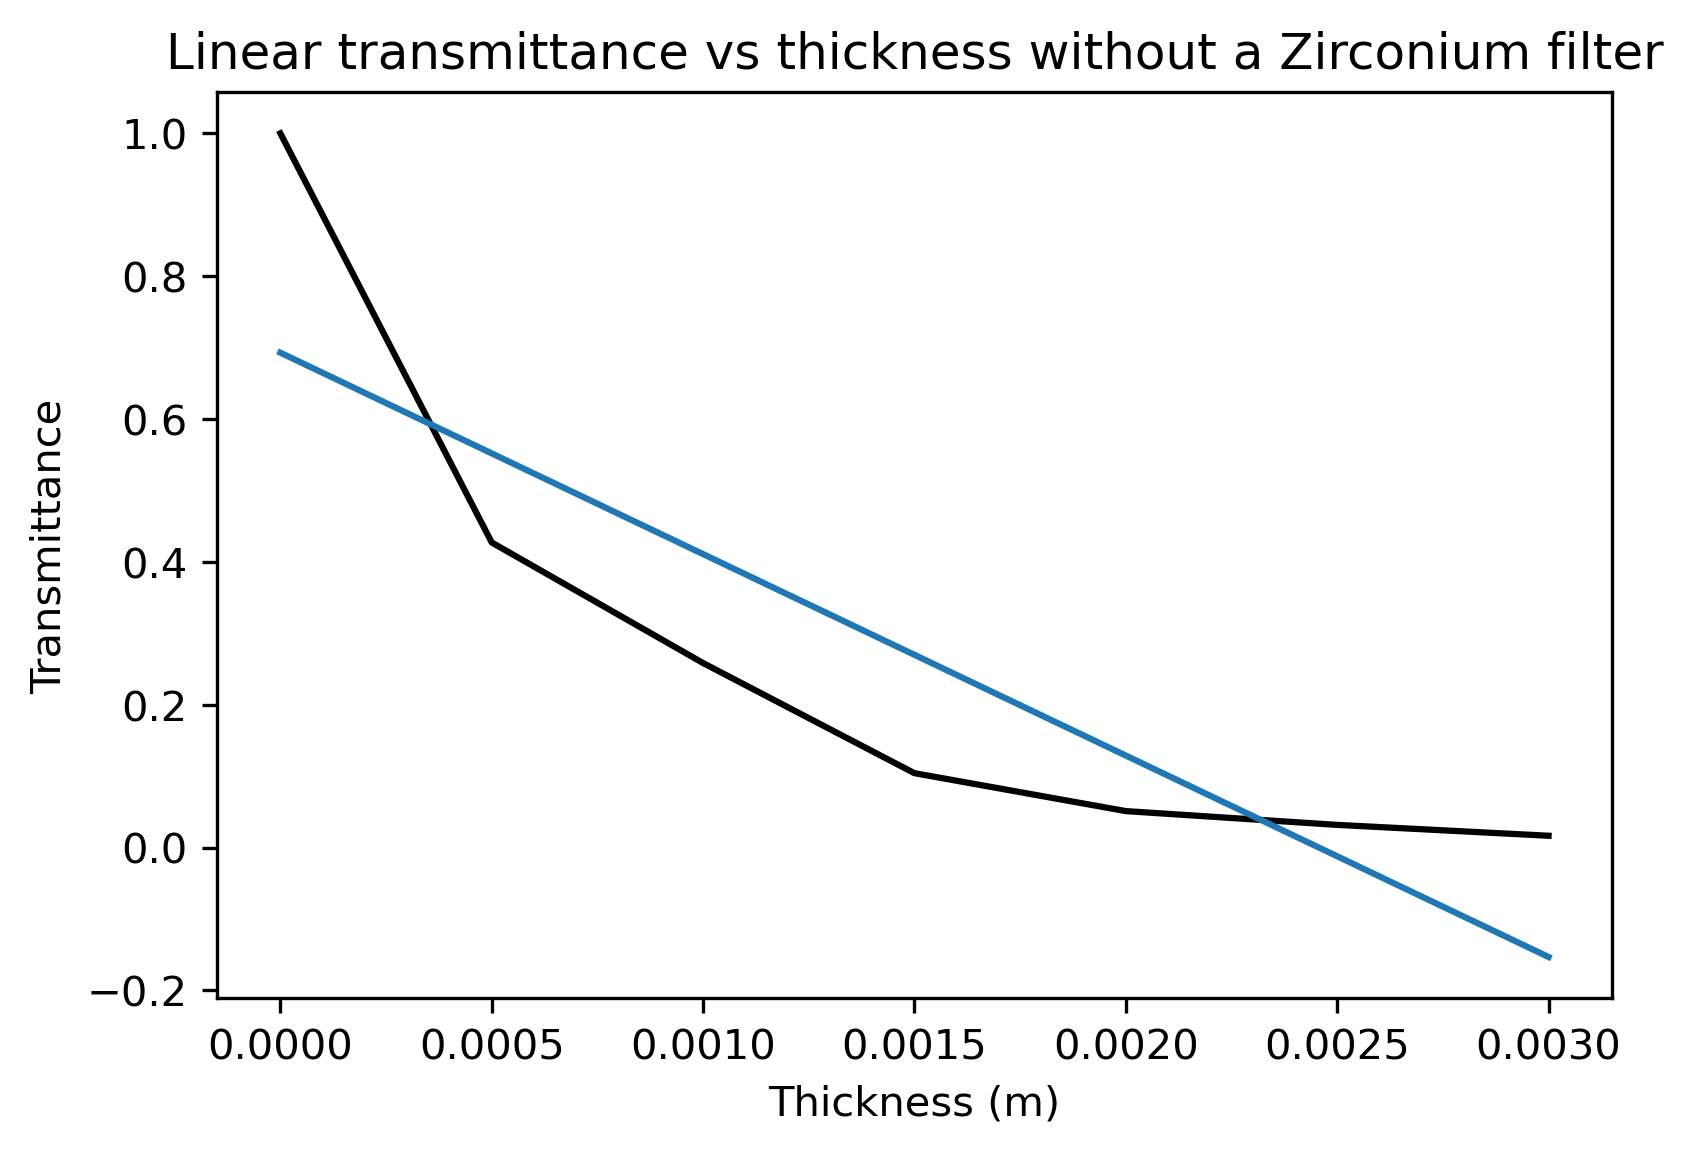
\includegraphics[scale=0.55]{Images/Report/Linear transmittance vs thickness without a Zirconium filter.png}
\caption{Linear plot showing the transmittance vs thickness without a zirconium filter. }
\label{Linear Thick No Filter}
\end{figure}

\begin{figure}[H]
\centering
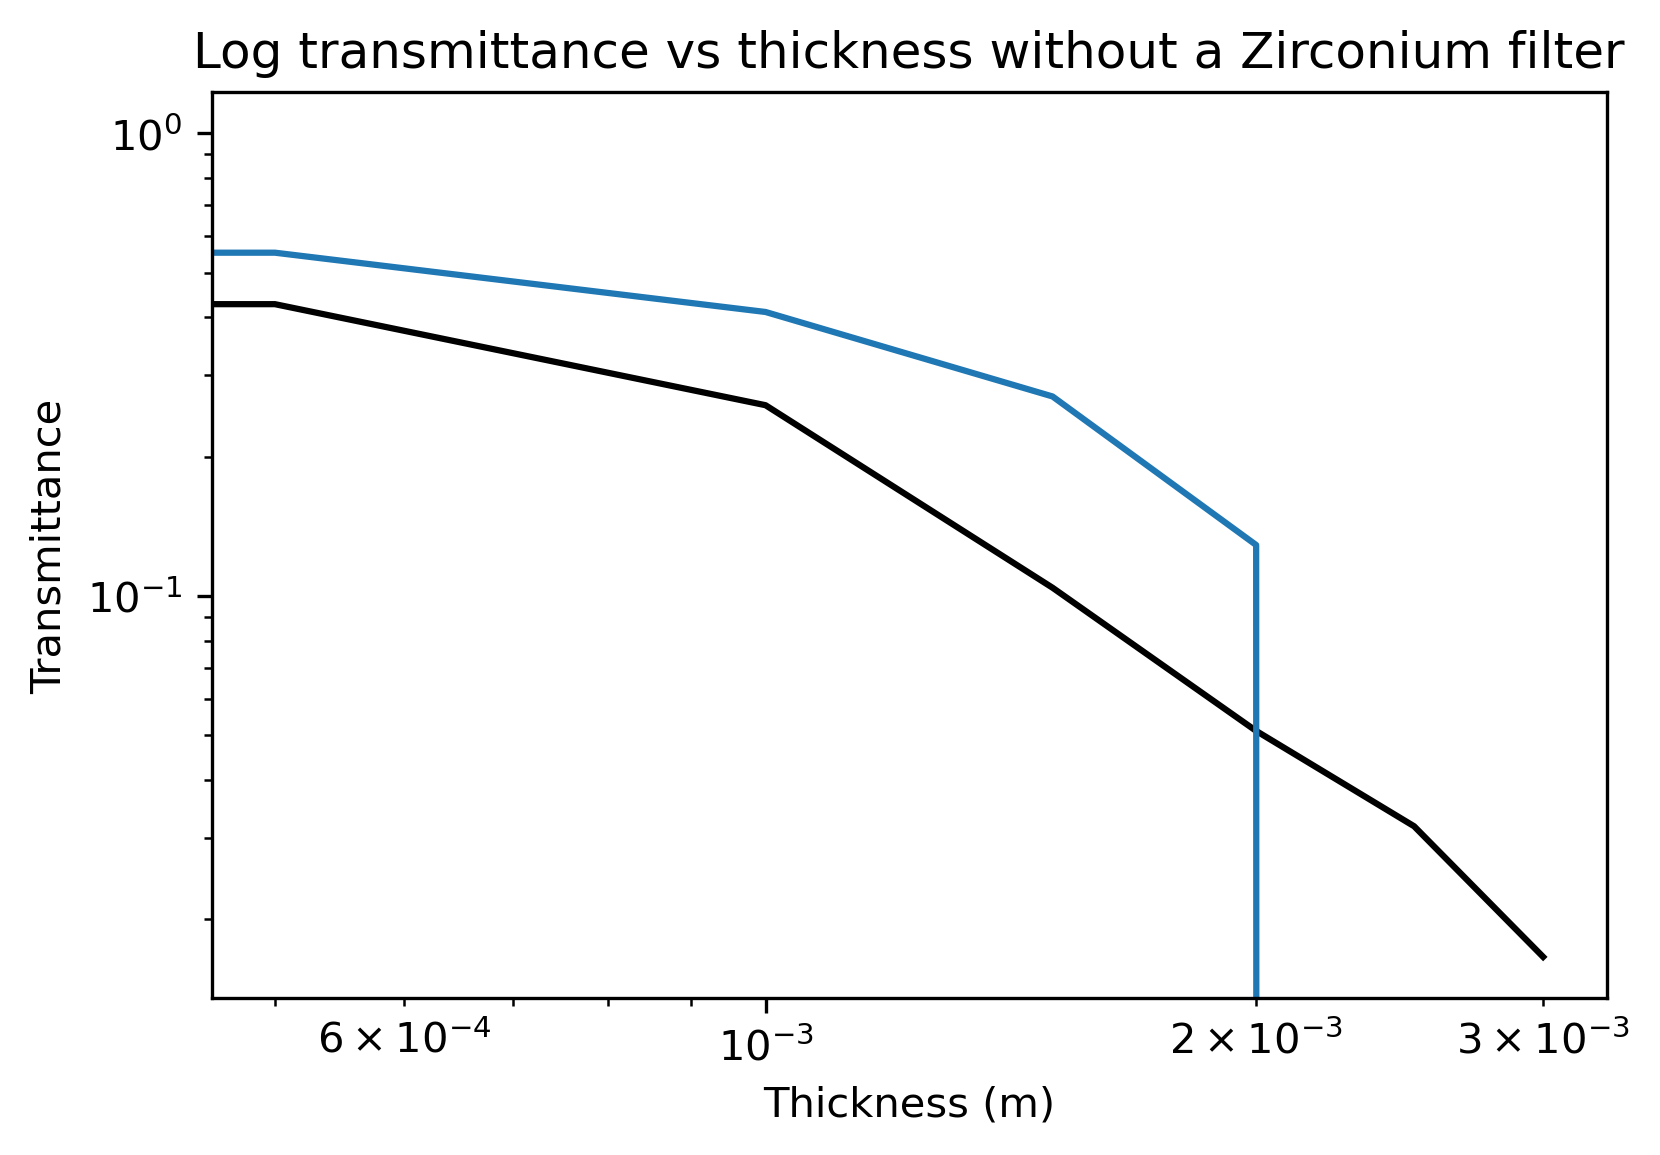
\includegraphics[scale=0.55]{Images/Report/Log transmittance vs thickness without a Zirconium filter.png}
\caption{Log plot showing the transmittance vs thickness without a zirconium filter. }
\label{Log Thick No Filter}
\end{figure}
\end{multicols}

\begin{multicols}{2}
\begin{figure}[H]
\centering
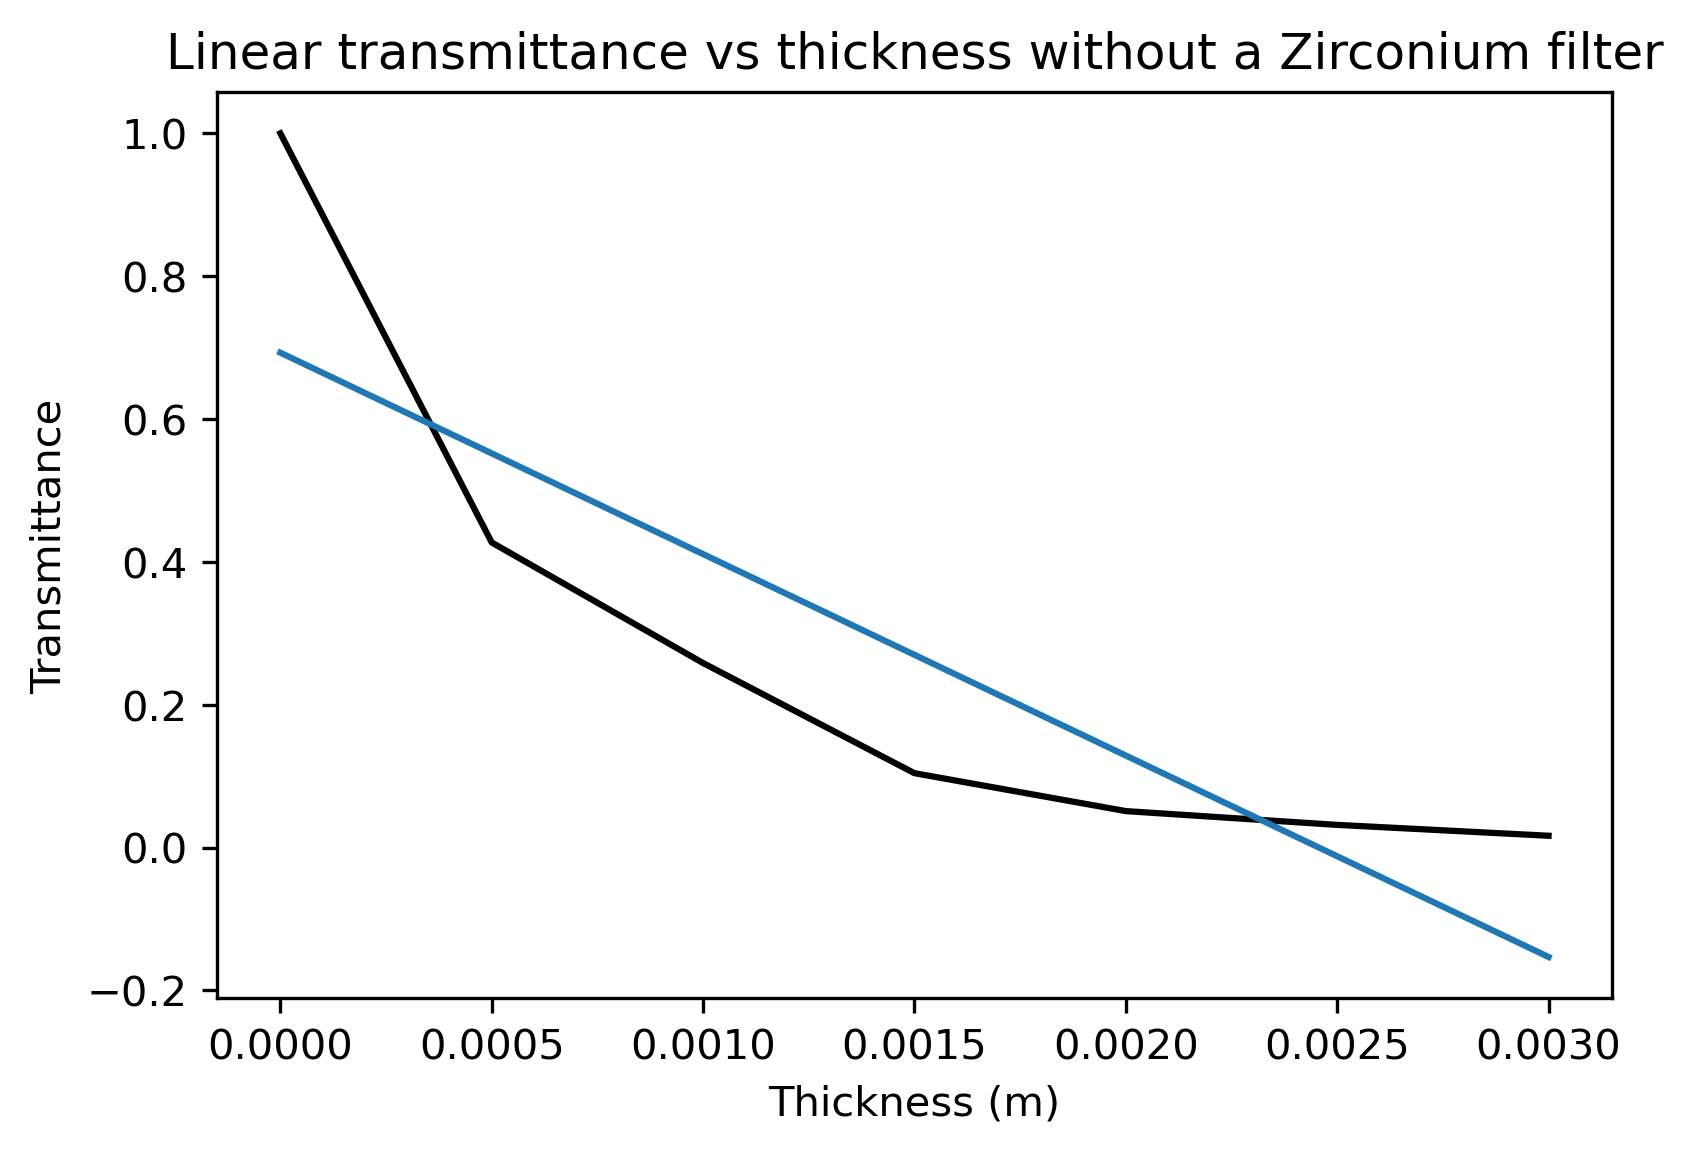
\includegraphics[scale=0.55]{Images/Report/Linear transmittance vs thickness without a Zirconium filter.png}
\caption{Linear plot showing the transmittance vs thickness with a zirconium filter. }
\label{Linear Thick Filter}
\end{figure}

\begin{figure}[H]
\centering
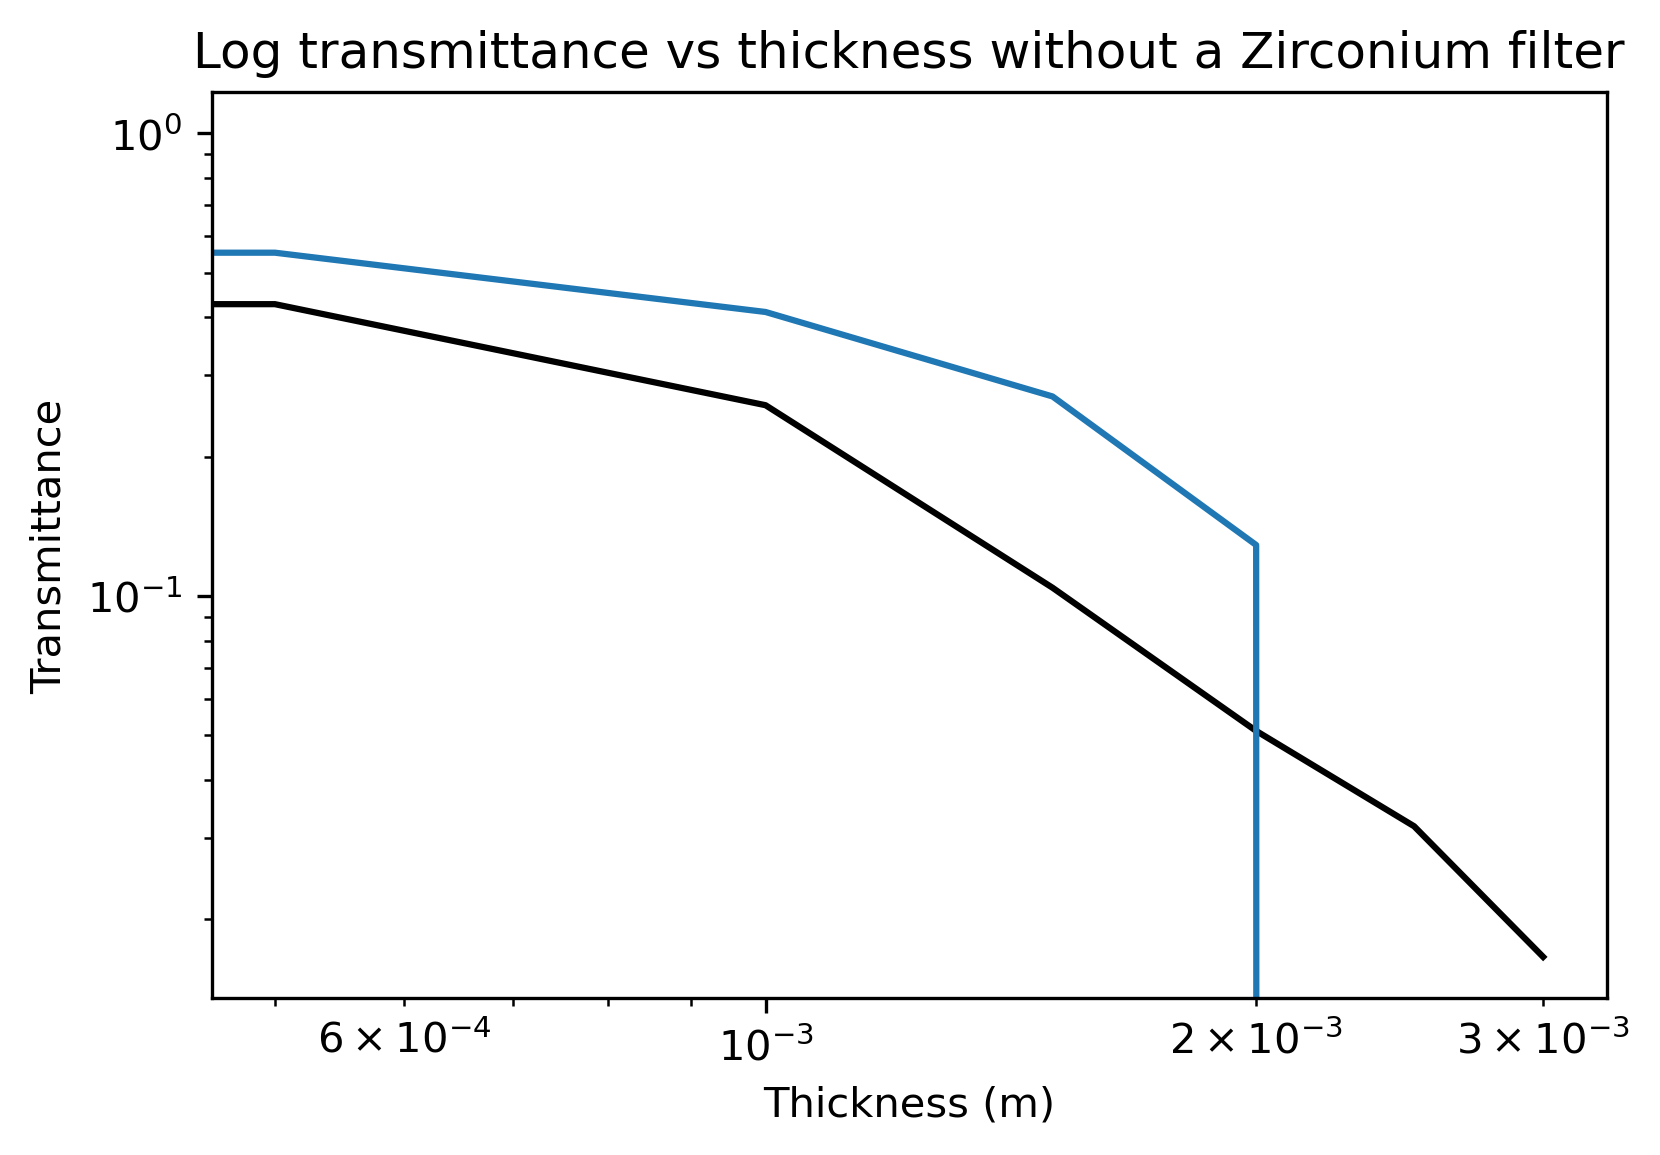
\includegraphics[scale=0.55]{Images/Report/Log transmittance vs thickness without a Zirconium filter.png}
\caption{Log plot showing the transmittance vs thickness with a zirconium filter. }
\label{Log Thick Filter}
\end{figure}
\end{multicols}

Plotting the the transmittance vs thickness data on a linear scale using \cref{Transmittance} for both without the Zirconium filter in \cref{Linear Thick No Filter} and with the filter in \cref{Linear Thick Filter} and then plotting the log scaled transmittance vs thickness data and with and without the filter in \cref{Log Thick No Filter} and \cref{Log Thick Filter} respectively. Its possible to see from the graph but mainly from \cref{Thickness Transmittance} that the Zirconium filter reduces the number of counts.

\begin{table}[H]
\begin{center}
 \footnotesize
 \begin{tabular}{|c|c||c|c|}
 \hline
 \multicolumn{2}{|c|}{Without Zirconium Filter} & \multicolumn{2}{|c|}{With Zirconium Filter} \\
 \hline 
 Thickness (m) & Transmittance & Thickness & Transmittance\\
 \hline \hline
  0.0000  & 0.0000 & 0.0000 & 0.0000 \\
  \hline
  0.0005 & 0.4272 & 0.0005 & 0.4026 \\
 \hline 
  0.0010  & 0.2584 & 0.0010 & 0.1890   \\
 \hline
  0.0015  & 0.1042 & 0.0015 & 0.0842  \\
 \hline 
  0.0020  & 0.0511 & 0.0020 & 0.0345  \\
 \hline
  0.0025  & 0.0318 & 0.0025 & 0.0189  \\
 \hline 
  0.0030  & 0.0196 & 0.0030 & 0.0093  \\
 \hline
 \end{tabular} \\ 
 \caption{Transmittance calculated by \cref{Transmittance} for both with and without Zirconium filter for different material thicknesses.}
 \label{Thickness Transmittance}
\end{center}
\end{table}

The linear L.A.C without the Zirconium filter 282.02 $\pm75.090$ and the log L.A.C without the Zirconium filter is 282.02. \\

The linear L.A.C with the Zirconium filter 278.85 $\pm81.912$ and the log L.A.C with the Zirconium filter is 278.85. \\

Looking at both values of the gradients of the the graphs, its clear to see that the Zirconium filter effects the counts as the filter absorbs or reflects the rays, this is due to Zirconium's high atomic number as it holds more electrons and absorbs or destroys the incoming x-rays as it penetrates the material.\\

%---------------------------------------------------------------------------
\subsection{Attenuation as a function of the absorber material}
\label{EAttenuation as a function of the absorber material SubSection}

Setting the voltage to U = 30kV, I = 0.02mA, $\Delta \beta$=0$^{\circ}$ and $\Delta$t = 30s \cite{Exp.D-2020}

\begin{table}[H]
\begin{center}
 \footnotesize
 \begin{tabular}{|c||c||c|c||c|c|}
 \hline
 \multicolumn{6}{|c|}{Attenuation as a function of absorber material without a Zirconium filter} \\
 \hline 
 Material & Angle & 1st Counts/s & 2nd Counts/s & Mean Counts/s & Sigma\\
 \hline \hline
  No Material & 0 & 1738.00 & 1867.00 & 1825.00 & $\pm$42.72 \\
 \hline
  Carbon & 10 & 1728.00 & 1815.00 & 1771.50 & $\pm$42.09 \\
 \hline 
  Aluminium & 20 & 1072.00 & 1145.50 & 1108.75 & $\pm$35.30 \\
 \hline \hline
 \multicolumn{6}{|c|}{ Change settings to U = 30kV, I = 1.0mA, $\Delta$t = 300s} \\
  \hline 
  Material & Angle & 1st Counts/s & 2nd Counts/s & Mean Counts/s & Sigma\\
 \hline \hline
  Iron & 30 & 205.80 & 142.00 & 173.90 & $\pm$13.19 \\
 \hline
  Copper & 40 & 24.08 & 56.00 & 40.04 & $\pm$6.33 \\
 \hline 
  Zirconium & 50 & 151.80 & 173.10 & 162.45 & $\pm$12.75\\
 \hline 
  Silver & 60 & 51.68 & 56.60 & 54.09 & $\pm$7.35 \\
 \hline 
 \end{tabular} \\ 
 \caption{Mean counts measured through different materials without a Zirconium filter.}
 \label{Material No Filter}
\end{center}
\end{table}

Setting the voltage to U = 30kV, I = 0.02mA, $\Delta \beta$=0$^{\circ}$ and $\Delta$t = 30s \cite{Exp.D-2020}


\begin{table}[H]
\begin{center}
 \footnotesize
 \begin{tabular}{|c||c||c|c||c|c|}
 \hline
 \multicolumn{6}{|c|}{Attenuation as a function of absorber material with a Zirconium filter} \\
 \hline 
 Material & Angle & 1st Counts/s & 2nd Counts/s & Mean Counts/s & Sigma\\
 \hline \hline
  No Material & 0 & 640.00 & 889.50 & 764.75 & $\pm$27.65 \\
 \hline
  Carbon & 10 & 616.90 & 863.70 & 740.30 & $\pm$27.21 \\
 \hline 
  Aluminium & 20 & 348.20 & 487.20 & 417.70 & $\pm$20.44 \\
 \hline \hline
 \multicolumn{6}{|c|}{ Change settings to U = 30kV, I = 1.0mA, $\Delta$t = 300s} \\
  \hline 
  Material & Angle & 1st Counts/s & 2nd Counts/s & Mean Counts/s & Sigma\\
 \hline \hline
  Iron & 30 & 64.95 & 101.40 & 83.18 & $\pm$9.12 \\
 \hline
  Copper & 40 & 8.51 & 12.79 & 10.65 & $\pm$3.26 \\
 \hline 
  Zirconium & 50 & 87.77 & 116.40 & 102.09 & $\pm$10.1\\
 \hline 
  Silver & 60 & 11.50 & 16.94 & 14.22 & $\pm$3.77 \\
 \hline 
 \end{tabular} \\ 
 \caption{Mean counts measured through different materials with a Zirconium filter.}
 \label{Material Filter}
\end{center}
\end{table}

Setting the voltage to U = 0kV, I = 0.0mA, $\Delta \beta$=0$^{\circ}$ and $\Delta$t = 300s \cite{Exp.D-2020}


\begin{table}[H]
\begin{center}
 \footnotesize
 \begin{tabular}{|c||c|c||c|c|}
 \hline
 \multicolumn{5}{|c|}{Measuring the background radiation} \\
 \hline 
 Zirconium Filter & 1st Counts/s & 2nd Counts/s & Mean Counts/s & Sigma\\
 \hline \hline
  Without & 0.209 & 0.186 & 0.20 & $\pm$0.045 \\
 \hline
  With  & 0.233 & 0.196 & 0.21 & $\pm$0.046 \\
 \hline 
 \end{tabular} \\ 
 \caption{Mean counts measuring the background radiation with and without a Zirconium filter.}
 \label{Background Radiation}
\end{center}
\end{table}

\begin{multicols}{2}
\begin{figure}[H]
\centering
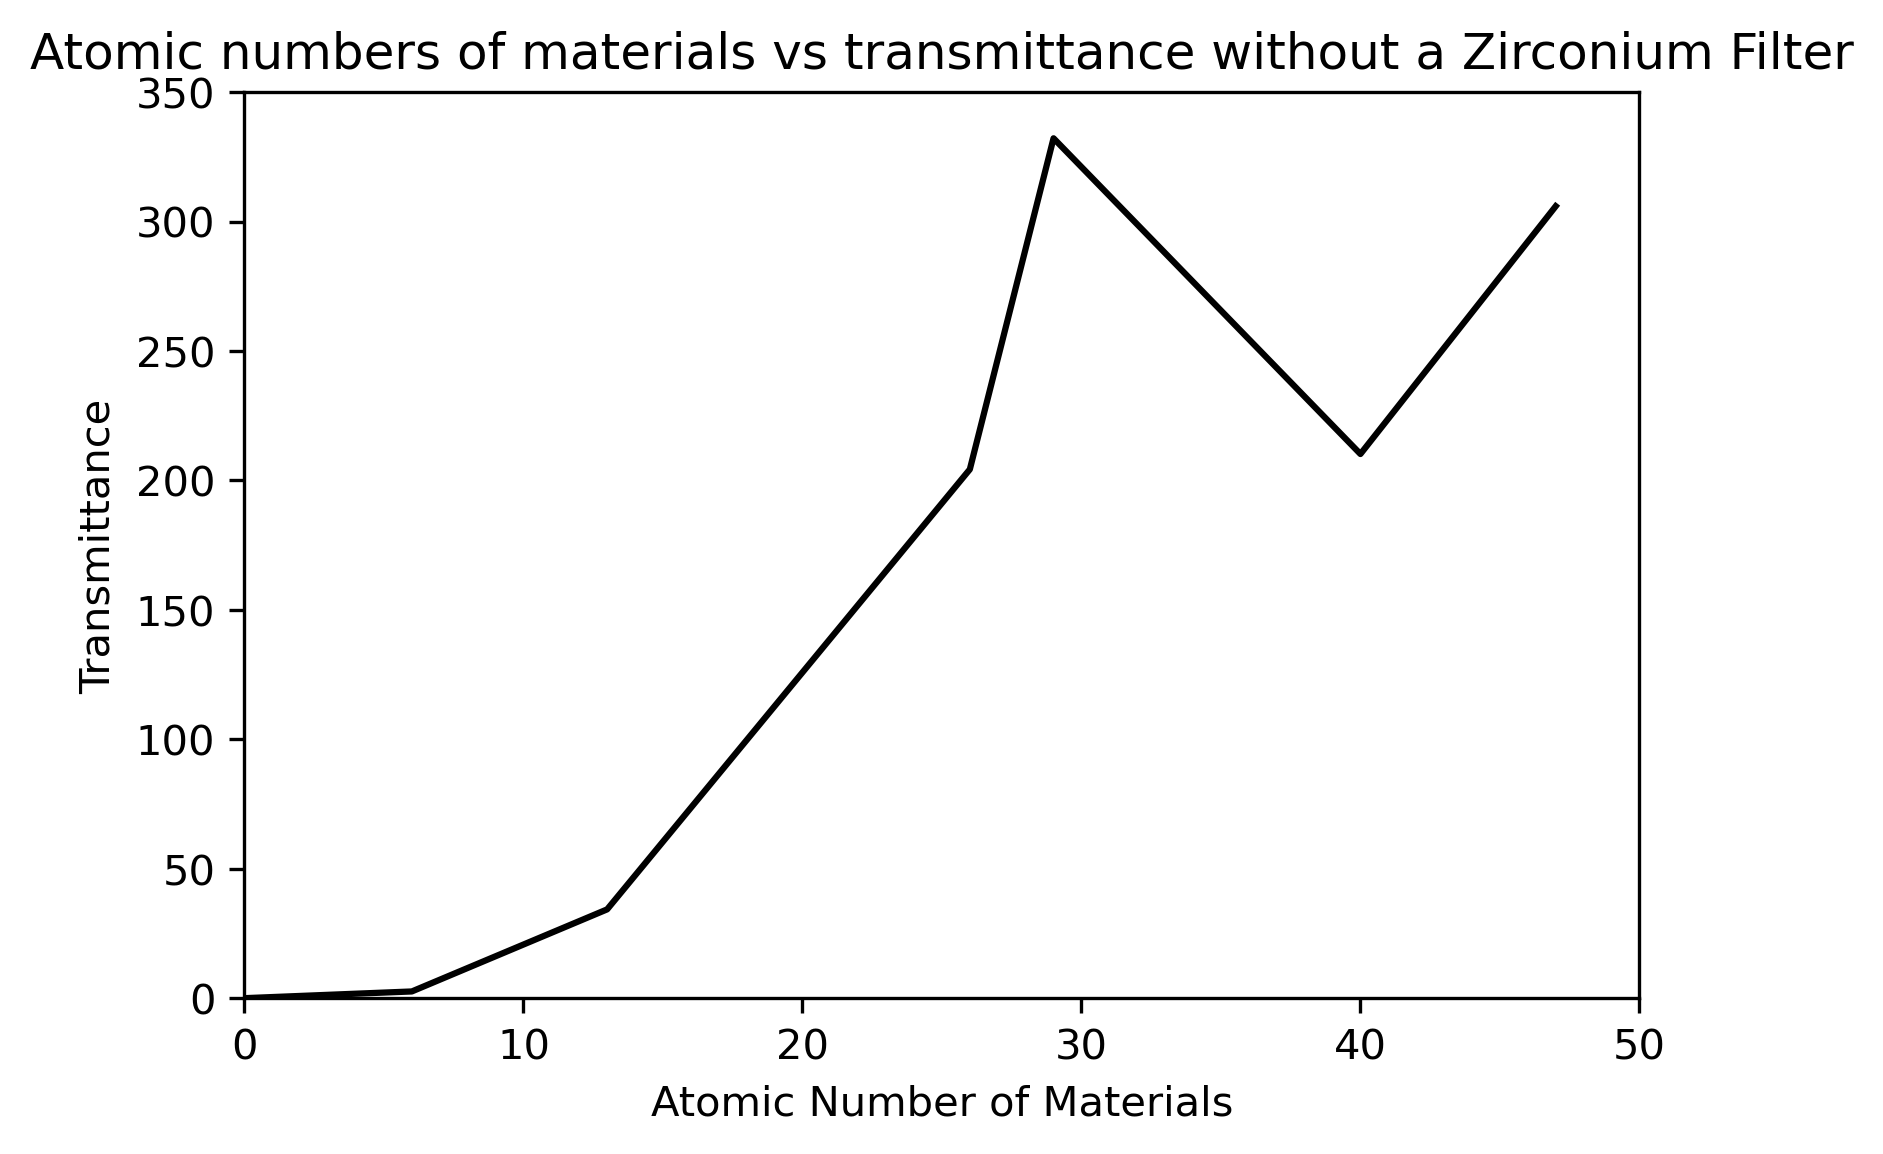
\includegraphics[scale=0.55]{Images/Report/Atomic numbers of materials vs transmittance without a Zirconium Filter.png}
\caption{Linear plot showing a calculated $\mu$ vs Atomic Number of each material without a Zirconium filter.}
\label{Absrober 2}
\end{figure}

\begin{figure}[H]
\centering
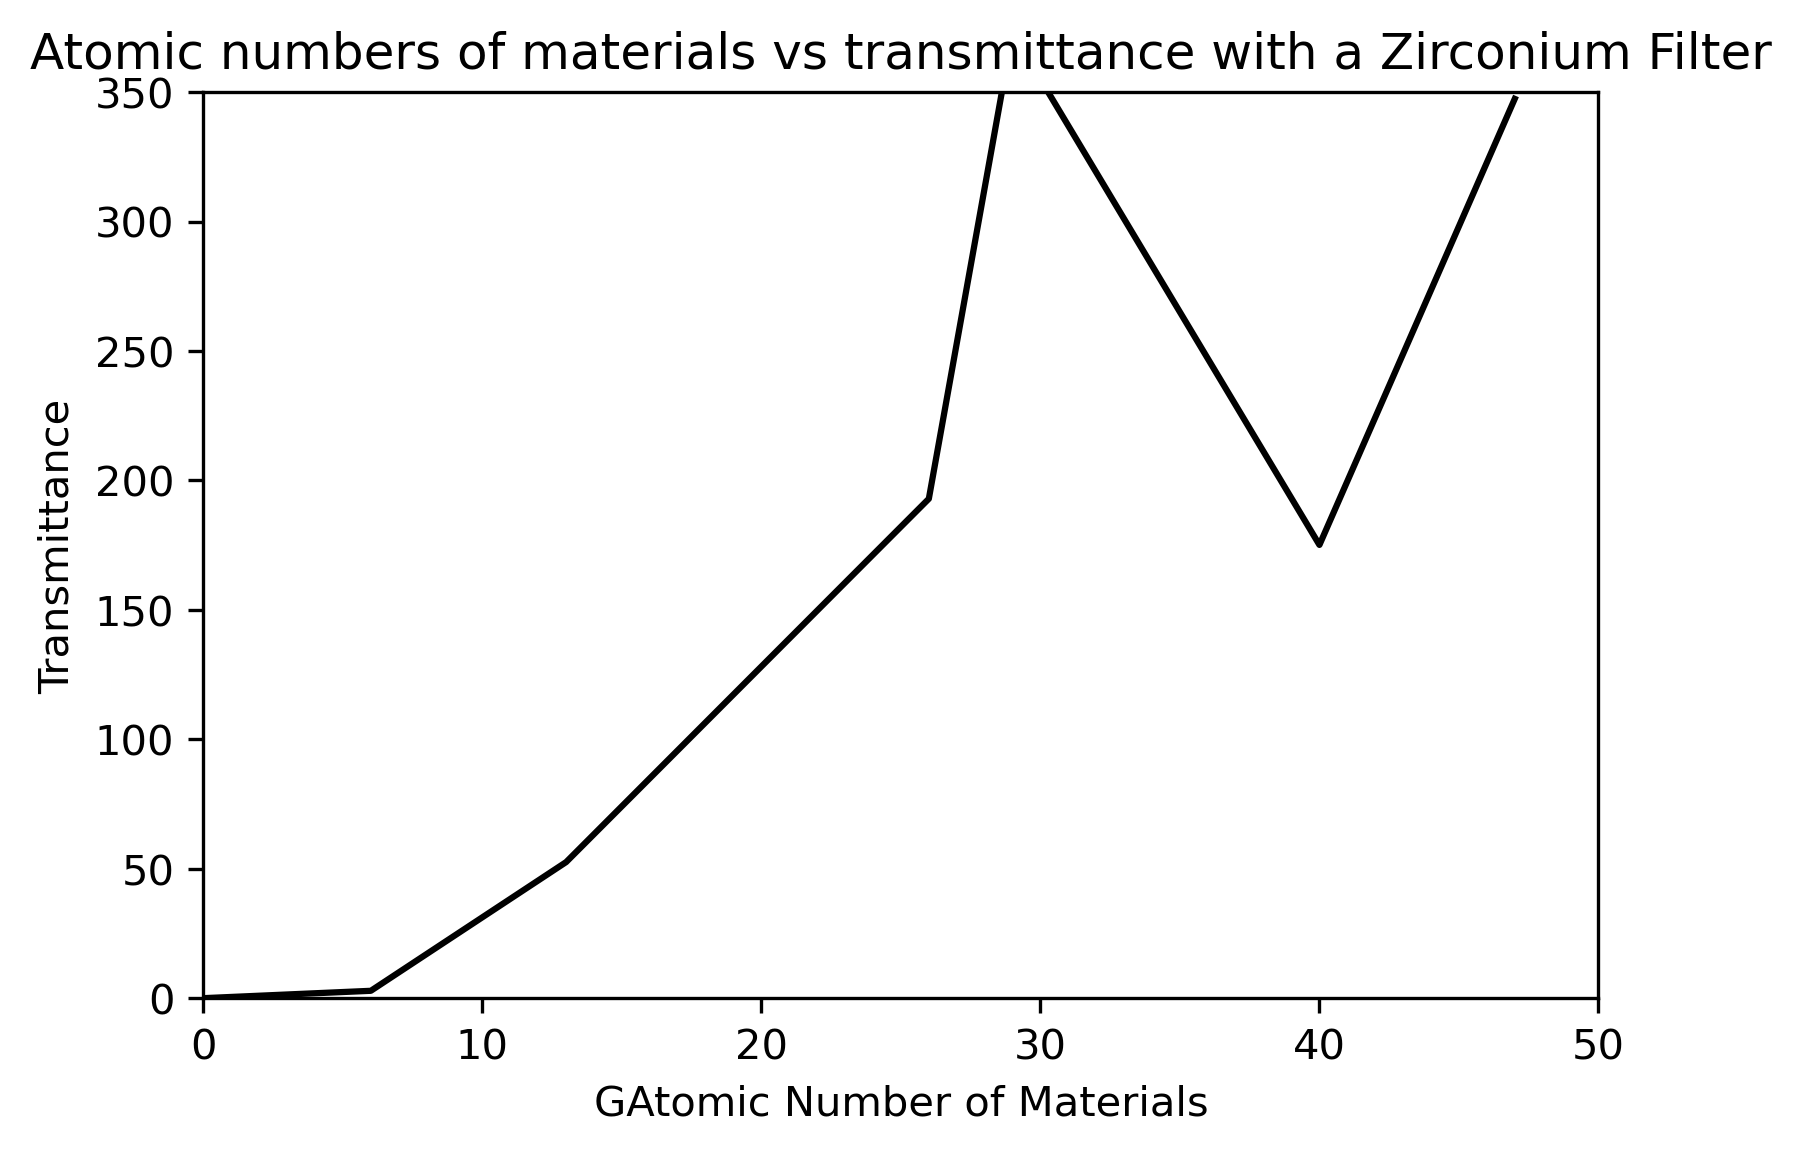
\includegraphics[scale=0.55]{Images/Report/Atomic numbers of materials vs transmittance with a Zirconium Filter.png}
\caption{Linear plot showing a calculated $\mu$ vs Atomic Number of each material with a Zirconium filter.}
\label{Absorber 2}
\end{figure}
\end{multicols}

In this case plotting the estimated value of $\mu$ calculated by \cref{Log Tramsittance} vs the atomic number showing in \cref{Absorber Transmittance}its clear to see that Zirconium is a good absorber of x-rays much like lead is with gamma-rays, though its interesting to see that even with the Zirconium filter copper is highly absorbent. 

\begin{table}[H]
\begin{center}
 \footnotesize
 \begin{tabular}{|c|c||c|c|c||c|c|c|}
 \hline
 \multicolumn{2}{|c|}{Absorber Transmittance} & \multicolumn{3}{|c|}{Without Zirconium Filter} & \multicolumn{3}{|c|}{With Zirconium Filter} \\
 \hline 
 Material & Atomic No. & Transmittance & L.A.C & Sigma & Transmittance & L.A.C & Sigma \\
 \hline \hline
  No Material  & 0 & 1.000 & 0 & 0 &1.000 & 0& 0 \\
  \hline
  Carbon & 6 & 0.9706 & 2.59 & 1.61 & 0.9678 & 2.85 & 1.69 \\
 \hline 
  Aluminium  & 13 & 0.6074 & 43.30 & 6.58 & 0.5459 & 52.57 & 7.25  \\
 \hline
  Iron  & 26 & 0.0952 & 204.29 & 14.29 & 0.1085 & 192.92 & 13.89\\
 \hline 
  Copper  & 29 & 0.0218 & 312.19 & 18.23 & 0.0136 & 372.98 & 19.31\\
 \hline
  Zirconium  & 40 & 0.0899 & 210.22 & 14.50 & 0.1332 & 175.09 & 13.23  \\
 \hline 
  Silver & 47 & 0.0295 & 305.95 & 17.49 & 0.0183 & 347.41 & 18.64  \\
 \hline
 \end{tabular} \\ 
 \caption{Transmittance calculated by \cref{Transmittance} for both with and without Zirconium filter for different absorber materials.}
 \label{Absorber Transmittance}
\end{center}
\end{table}

\begin{figure}[H]
\centering
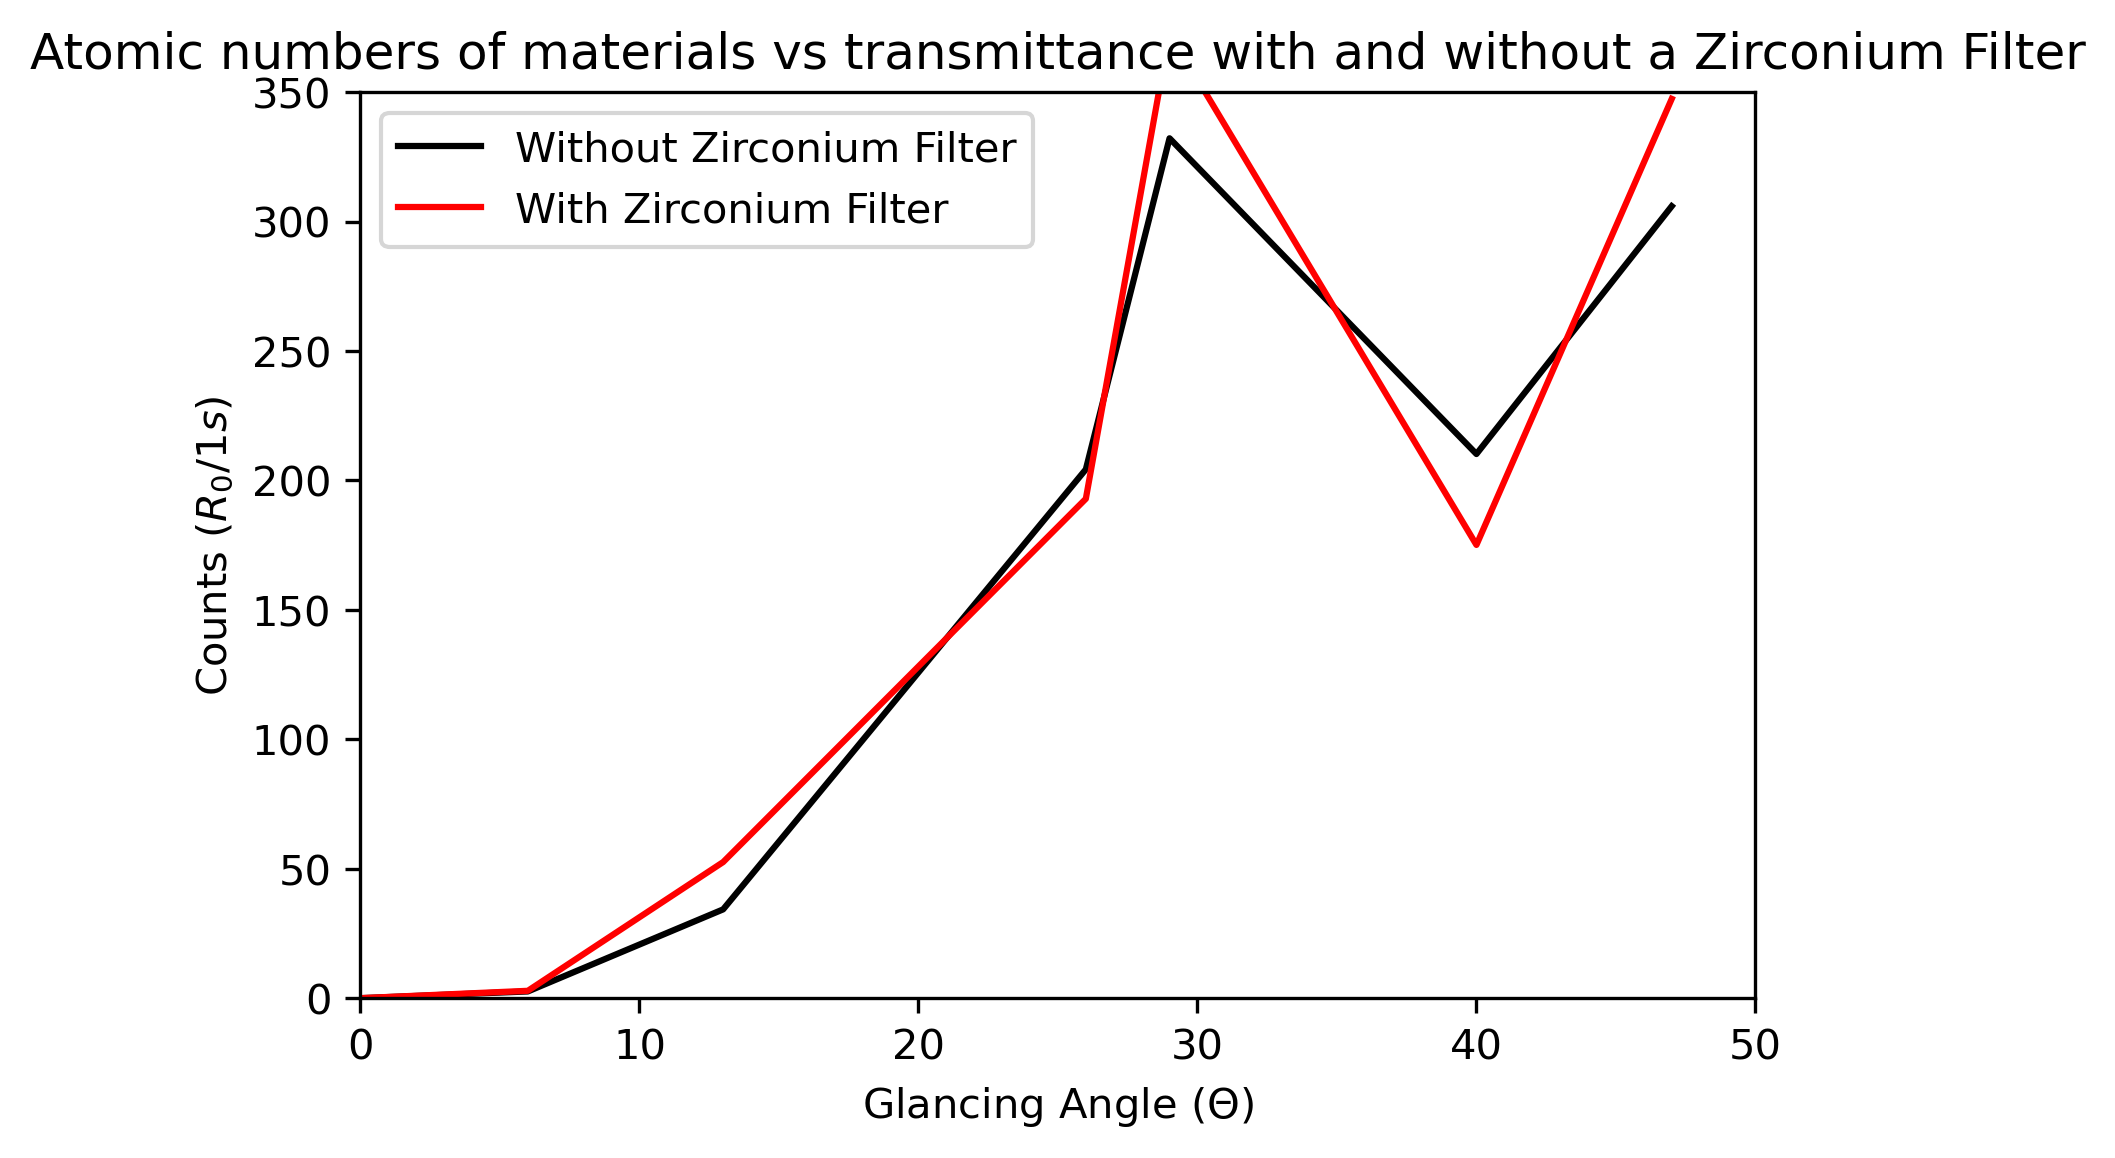
\includegraphics[scale=0.55]{Images/Report/Atomic numbers of materials vs transmittance with and without a Zirconium Filter.png}
\caption{Linear plot comparing the calculated $\mu$ vs Atomic Number of each material with and without a Zirconium filter.}
\label{Absrober 2}
\end{figure}

By comparing both sets of data with and without the Zirconium filter, \cref{Absrober 2} shows that the higher the atomic number the more resilient the absorption rate is and a lower transmittance is formed. Though however Zirconium is strong and radioactive material, these effects could hinder the ray photons ability to pass through to the detector.

%---------------------------------------------------------------------------
\subsection{Bragg reflection of an LiF monocrystal}
\label{Bragg reflection of an LiF monocrystal SubSection}

\begin{figure}[H]
\centering
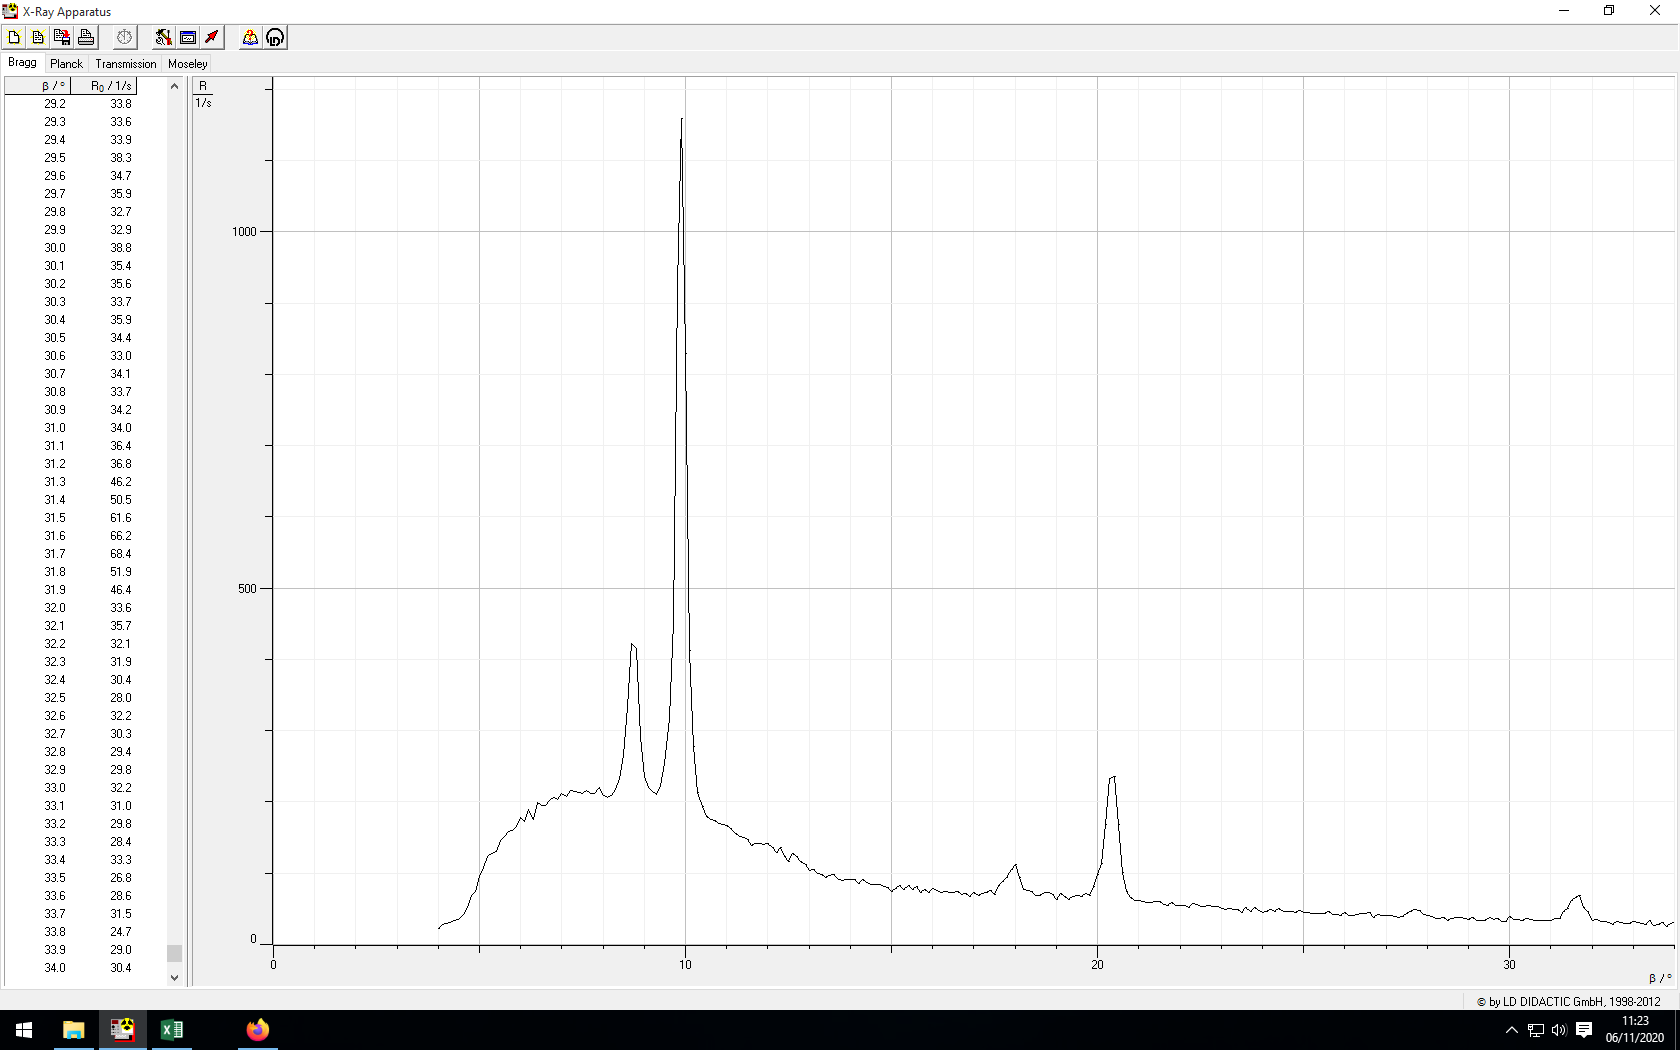
\includegraphics[scale=0.3]{Images/Report/LiF 10s.PNG}
\caption{Plot showing CASSY taking and plotting the data, this allows the alpha and beta peaks to be seen for the LiF crystal.}
\label{LiF graph}
\end{figure}

\begin{table}[H]
\begin{center}
 \footnotesize
 \begin{tabular}{|c|c||c|c||c||c|c|c|}
 \hline
 \multicolumn{8}{|c|}{Bragg reflection at an LiF monocrystal} \\
 \hline 
 Glancing Angle & Sigma & Sin$\theta$ & Sigma & n & $\dfrac{n\lambda}{pm}$ & n$\lambda$ & Sigma\\
 \hline \hline
  8.27 & 0.15 & 0.91 & -0.07 & 1 & 63.09 & 3.686 & -0.28 \\
  \hline
  9.89 & 0.15 & -0.45 & -0.12 & 1 & 71.08 & -1.808 & -0.52 \\
 \hline 
  17.94 & 0.19 & -0.78 & 0.13 & 2 & 126.18 & -3.180 & 0.52  \\
 \hline
  20.33 & 0.116 & 0.99 & 0.001 & 2 & 142.16 & 4.014 & 0.006\\
 \hline 
  27.71 & 0.12 & -0.105 & -0.105 & 3 & 189.27 & 2.156 & -0.42\\
 \hline
  31.61 & 0.16 & 0.153 & 0.153 & 3 & 213.24 & 0.777 & 0.62 \\
 \hline
 \end{tabular} \\ 
 \caption{Calculation of L.A.C for the Bragg reflection of an LiF monocrystal.}
 \label{Bragg LiF Reflection}
\end{center}
\end{table}

By using python to plot sin$\theta$ vs n$\lambda$ and also plot the gradient which equals to the linear attenuation coefficient which is estimated at a value of $\mu$ for the LiF monocrystal is 0.2481 $cm^{-1}$ $\pm$0.04 which does equal to the literature values of 4.03 $cm^{-1}$ \cite{CRC}. The $a_0$ value differs of that of the NaCl single crystal as the LiF monocrystal's lattice structure is that of body centered cubic means that the atomic structure of the inorganic element is designed as a cube with an additional support particle in the centre, this means that the LiF monocrystal is bad at diffracting the x-rays.

\begin{figure}[H]
\centering
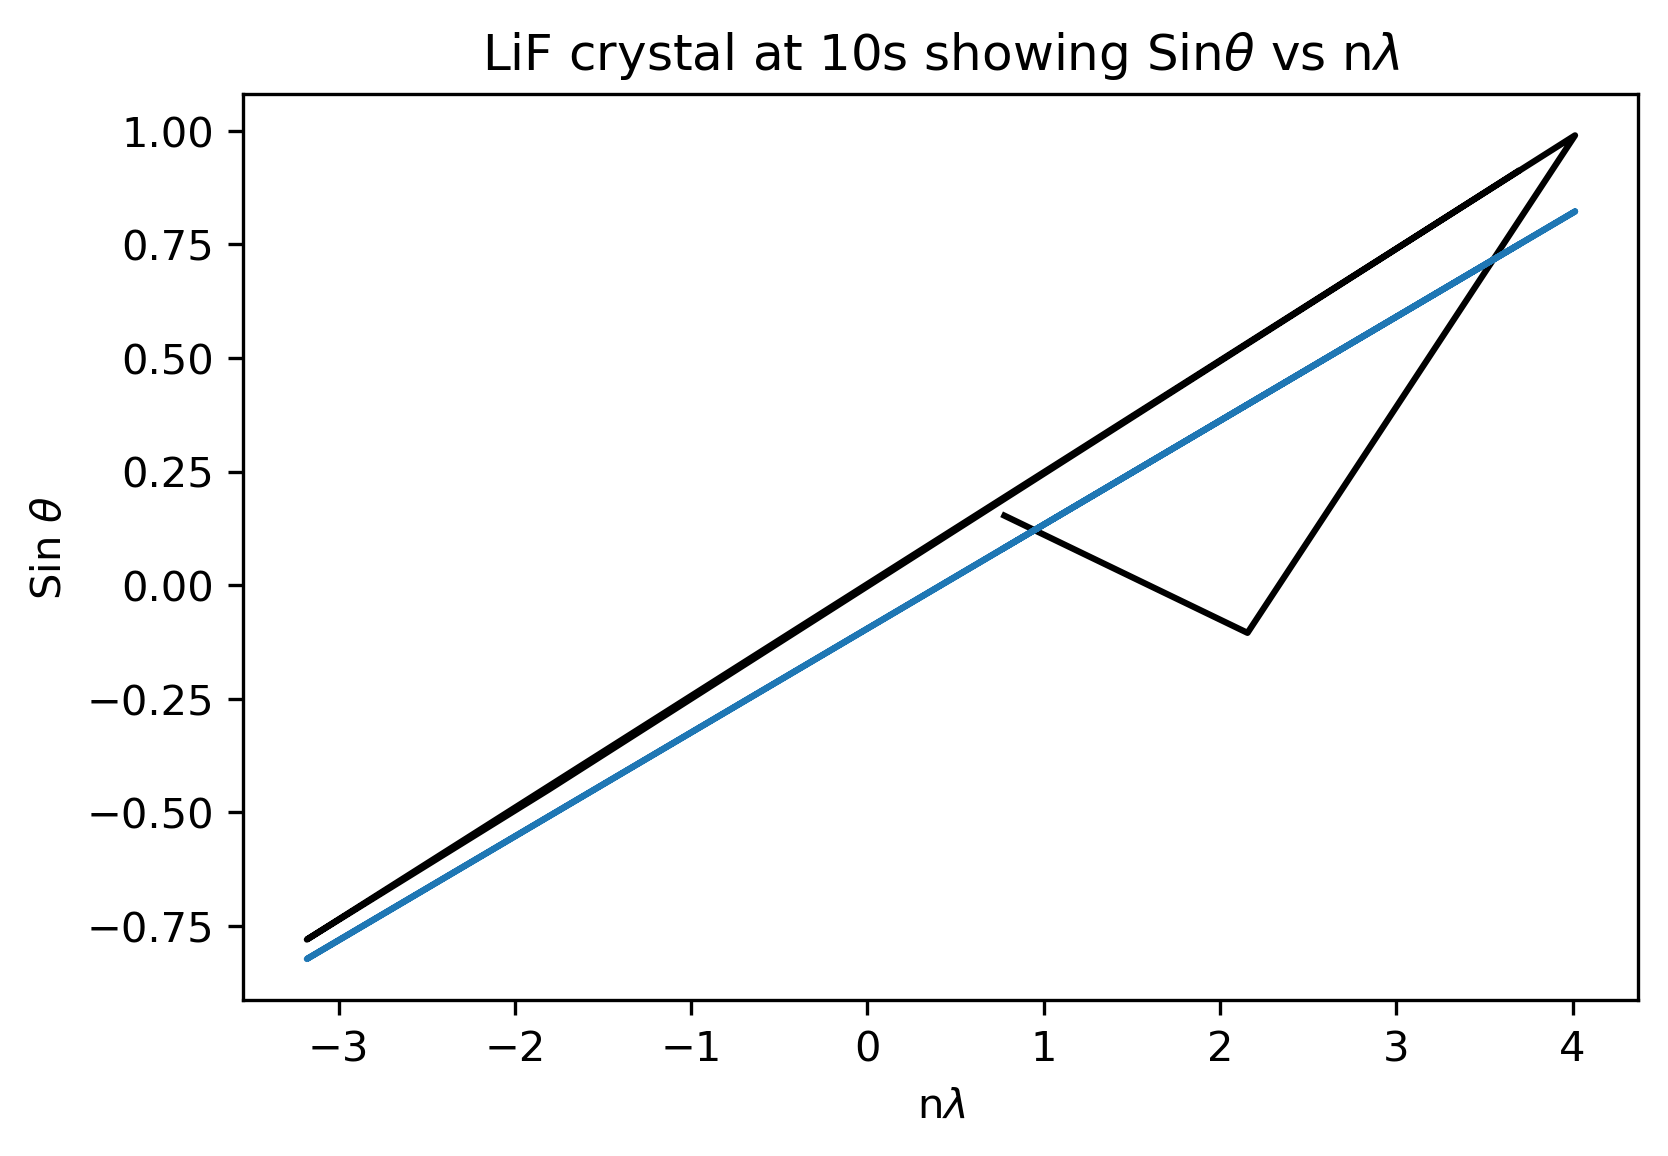
\includegraphics[scale=0.55]{Images/LIF10s.png}
\caption{Plot showing Sin$\theta$ vs n$\lambda$ that gives the gradients of the slope as the L.A.C for the LiFsingle crystal.}
\label{LiF graph 1}
\end{figure}

%---------------------------------------------------------------------------
\subsection{Bragg reflection of an NaCl single crystal}
\label{Bragg reflection of an NaCl single crystal SubSection}

\begin{figure}[H]
\centering
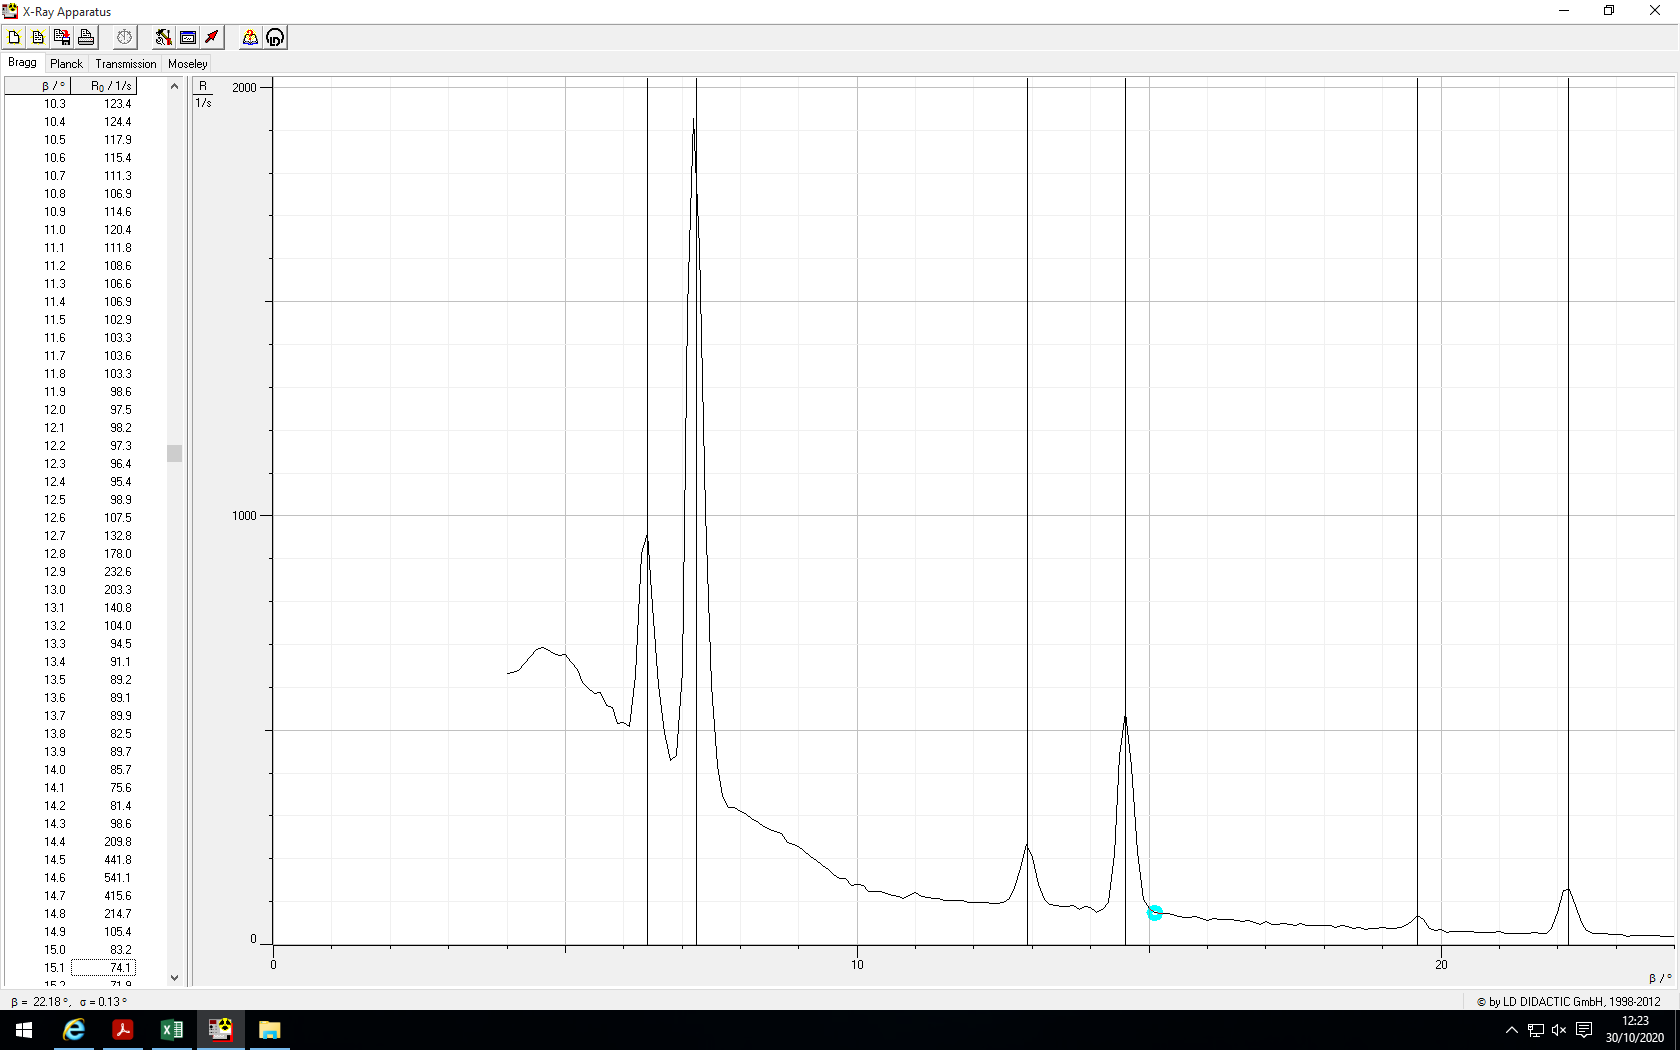
\includegraphics[scale=0.3]{Images/Report/NaC1 10s Centre.PNG}
\caption{Plot showing CASSY taking and plotting the data, this allows the alpha and beta peaks to be seen for the NaCl crystal.}
\label{NaCl graph}
\end{figure}


\begin{table}[H]
\begin{center}
 \footnotesize
 \begin{tabular}{|c|c||c|c||c||c|c|c|}
 \hline
 \multicolumn{8}{|c|}{Bragg reflection at an NaCl single crystal} \\
 \hline 
 Glancing Angle & Sigma & Sin$\theta$ & Sigma & n & $\dfrac{n\lambda}{pm}$ & n$\lambda$ & Sigma\\
 \hline \hline
  6.41 & 0.12 & 0.126 & 0.117 & 1 & 63.09 & 0.713 & 0.475 \\
  \hline
  9.24 & 0.13 & 0.817 & 0.068 & 1 & 71.08 & 4.609 & 0.273 \\
 \hline 
 12.94 & 0.12 & 0.365 & 0.068 & 2 & 126.18 & 2.059 & 0.436 \\
 \hline
  14.6 & 0.12 & 0.895 & -0.059 & 2 & 142.16 & 5.047 & -0.241\\
 \hline 
  19.6 & 0.10 & 0.682 & 0.682 & 3 & 189.27 & 3.846 & 0.281\\
 \hline
  22.18 & 0.13 & -0.0187 & -0.188 & 3 & 213.24 & -1.059 & -0.507 \\
 \hline
 \end{tabular} \\ 
 \caption{Calculation of L.A.C for the Bragg reflection of an NaCl single crystal.}
 \label{Bragg NaCl Reflection}
\end{center}
\end{table}

\begin{figure}[H]
\centering
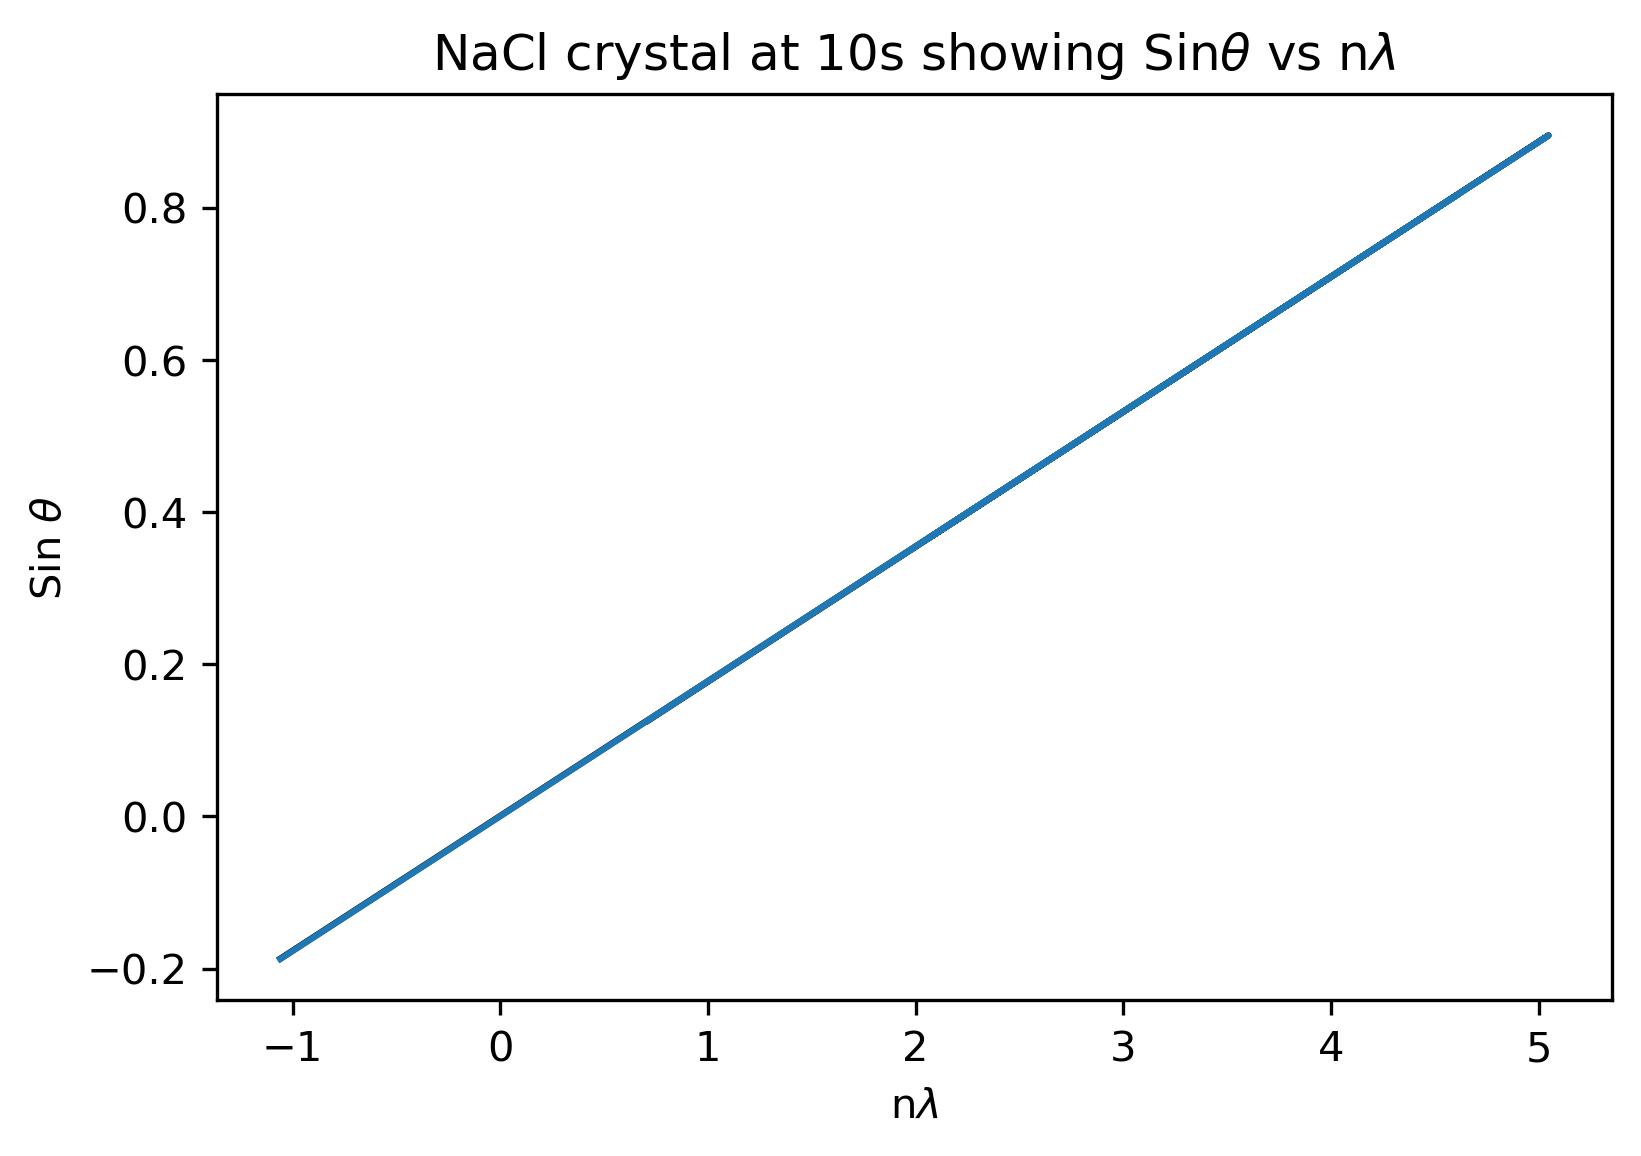
\includegraphics[scale=0.55]{Images/NACL10s.png}
\caption{Plot showing Sin$\theta$ vs n$\lambda$ that gives the gradients of the slope as the L.A.C for the NaCl single crystal.}
\label{NaCl graph1}
\end{figure}

The NaCl is face centred cubic which means an additional particle is place in line on the of its lattice structure meaning the x-rays cannot pass more easily through and reflects more x-rays, by observing \cref{NaCl graph1} the estimated value of $\mu$ for the NaCl single crystal is 0.1773 $cm^{-1}$ $\pm$7.75e$^{-5}$. Where as the literature value is 5.64$cm^{-1}$ \cite{CRC}.

%---------------------------------------------------------------------------
%	DISCUSSION
%---------------------------------------------------------------------------
\section{Discussion}
\label{Disscussion Section}

In this experiment, a lot of mathematics were used, the ability to use python and plot graphs together allows for more accurate results. The linear attenuation for thickness proved right for both the linear-linear scale and log-linear scale and ultimately led to proving that an increase in atomic number decreases the transmittance depending on the structure of the elements lattice planes. \\

For the Bragg reflection for the LiF monocrystal and the NaCl single crystal, though both graphs of $sin\theta$ vs n$\lambda$ were both linear as was requested, the wavelength was tricky to determine due to the pm element, though the result outputted in a y=mx+c format, finding the linear attenuation coefficient was straight forward though it did not match with the researched literature values in \cite{CRC}. \\

Though the experiment proved tricky mathematically in the graph plots, i believe further analysis would highlights errors in my calculations and also to not rely on python for doing almost all of them, this proved tricky to goes back and check my values. I would think for improvement is to observe the different materials at different thicknesses, especially with the Zirconium as seen the 0.0005m panel took a negative from the trend line and dropped almost a 1/4 to 0, further testing could indicate that a thicker piece could potentially absorb nearly all of the emitted rays much like the element lead does for gamma rays.

%---------------------------------------------------------------------------
%	CONCLUSION
%---------------------------------------------------------------------------
\section{Conclusion}
\label{Conclusion Section}

It has been proven that using different thicknesses of the same material can output the linear attenuation coefficient of that materials, though its transmittance is affected by and increase of decrease in thickness. Further more this linear attenuation coefficient proves helpful in determining which element absorbs the most x-rays and the least, essentially which element is a better attenuator.  \\

Further testing and investigation into the mathematics of finding the lattice constant for the Bragg reflection of an LiF monocrystal and NaCl single crystal, the values obtained were plotted linearly and the $\mu$ values calculated from the gradient of the slope of the linear plots were estimated as half of the literature values in \cite{CRC}.

%---------------------------------------------------------------------------
%	APPENDIX
%---------------------------------------------------------------------------
\newpage
\section{Appendix}
\label{Appendix Section}

\begin{figure}[H]
\centering
\includegraphics[scale=0.25]{Images/IMG_0412.PNG}
\end{figure}
\newpage
\begin{figure}[H]
\centering
\includegraphics[scale=0.25]{Images/IMG_0413.PNG}
\end{figure}
\newpage
\begin{figure}[H]
\centering
\includegraphics[scale=0.25]{Images/IMG_0414.PNG}
\end{figure}
\newpage
\begin{figure}[H]
\centering
\includegraphics[scale=0.25]{Images/IMG_0415.PNG}
\end{figure}
\newpage
\begin{figure}[H]
\centering
\includegraphics[scale=0.25]{Images/IMG_0416.PNG}
\end{figure}
\newpage
\begin{figure}[H]
\centering
\includegraphics[scale=0.25]{Images/IMG_0417.PNG}
\end{figure}
\newpage
\begin{figure}[H]
\centering
\includegraphics[scale=0.25]{Images/IMG_0418.PNG}
\end{figure}
\newpage
\begin{figure}[H]
\centering
\includegraphics[scale=0.25]{Images/IMG_0419.PNG}
\end{figure}
%---------------------------------------------------------------------------
%	REFERENCES
%---------------------------------------------------------------------------
\bibliographystyle{plain}
\bibliography{mybib.bib}
\end{document}